\documentclass[tikz,border=10pt]{standalone}
\usepackage{tikz}
\usepackage{amsmath}

\begin{document}

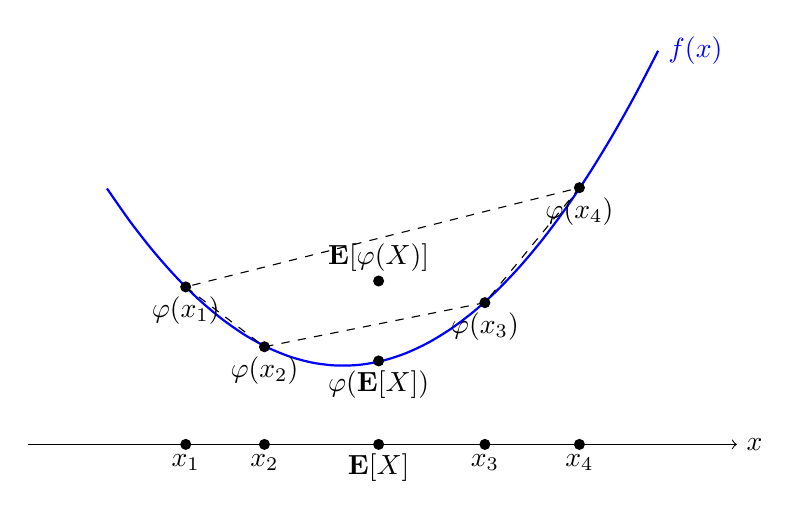
\begin{tikzpicture}[scale=2]
    \draw[->] (0, 0) -- (4.5, 0) node[right] {$x$};
    
    \draw[thick, domain=0.5:4, smooth, variable=\x, blue] plot ({\x}, {0.5*(\x-2)*(\x-2) + 0.5}) node[right] {$f(x)$};

    \fill (1.0,0) circle (1pt) node[below] {$x_1$};
    \fill (1.5,0) circle (1pt) node[below] {$x_2$};
    \fill (2.9,0) circle (1pt) node[below] {$x_3$};
    \fill (3.5,0) circle (1pt) node[below] {$x_4$};

    \fill (2.225,0) circle (1pt) node[below] {$\mathbf{E}[X]$};
    
    \fill (1.0,1.00) circle (1pt) node[below] {$\varphi(x_1)$};
    \fill (1.5,0.62) circle (1pt) node[below] {$\varphi(x_2)$};
    \fill (2.9,0.90) circle (1pt) node[below] {$\varphi(x_3)$};
    \fill (3.5,1.63) circle (1pt) node[below] {$\varphi(x_4)$};

    \fill (2.225,0.53) circle (1pt) node[below] {$\varphi(\mathbf{E}[X])$};

    \draw[dashed] (1.0,1.00) -- (1.5,0.62) -- (2.9,0.90) -- (3.5,1.63) -- (1.0,1.00);

    \fill (2.225,1.0375) circle (1pt) node[above] {$\mathbf{E}[\varphi(X)]$};


\end{tikzpicture}

\end{document}